\chapter*{Annexe 4}
\label{annexe:planning}
\addcontentsline{toc}{chapter}{Annexe 4}

%changer le format des sections, subsections pour apparaittre sans le num de chapitre
\makeatletter
\renewcommand{\thesection}{\@arabic\c@section}
\makeatother

%recommencer la numérotation des section à "1"
\setcounter{section}{0}

\section{Planning hebdomadaire}

Cette annexe restitue les éléments de planification hebdomadaire mis en place pour ce projet. 
Pour des raisons de présentation au sein de ce document, le planning a été scindé selon les parties suivantes : 

\begin{itemize}
 \item un aperçu global du planning, excluant le nom des tâches et intégrant les jalons, dead-lines et incréments produits clés 
 \item une présentation détaillée des tâches de réalisations documentaires, et de préparation de l'environnement de travail
 \item une présentation détaillée des tâches d'étude et des tâches de réalisation liées à ROS
 \item une présentation détaillée des tâches de réalisation liées à l'IHM, d'automatisation, de gestion de versions et de tâches annexes 
\end{itemize}

Les versions du système répondent au code couleurs suivant : gris correspond aux tâches effectuées avant la première release, violet après la première et bleu après la seconde. 

\begin{sidewaysfigure}
\centering
    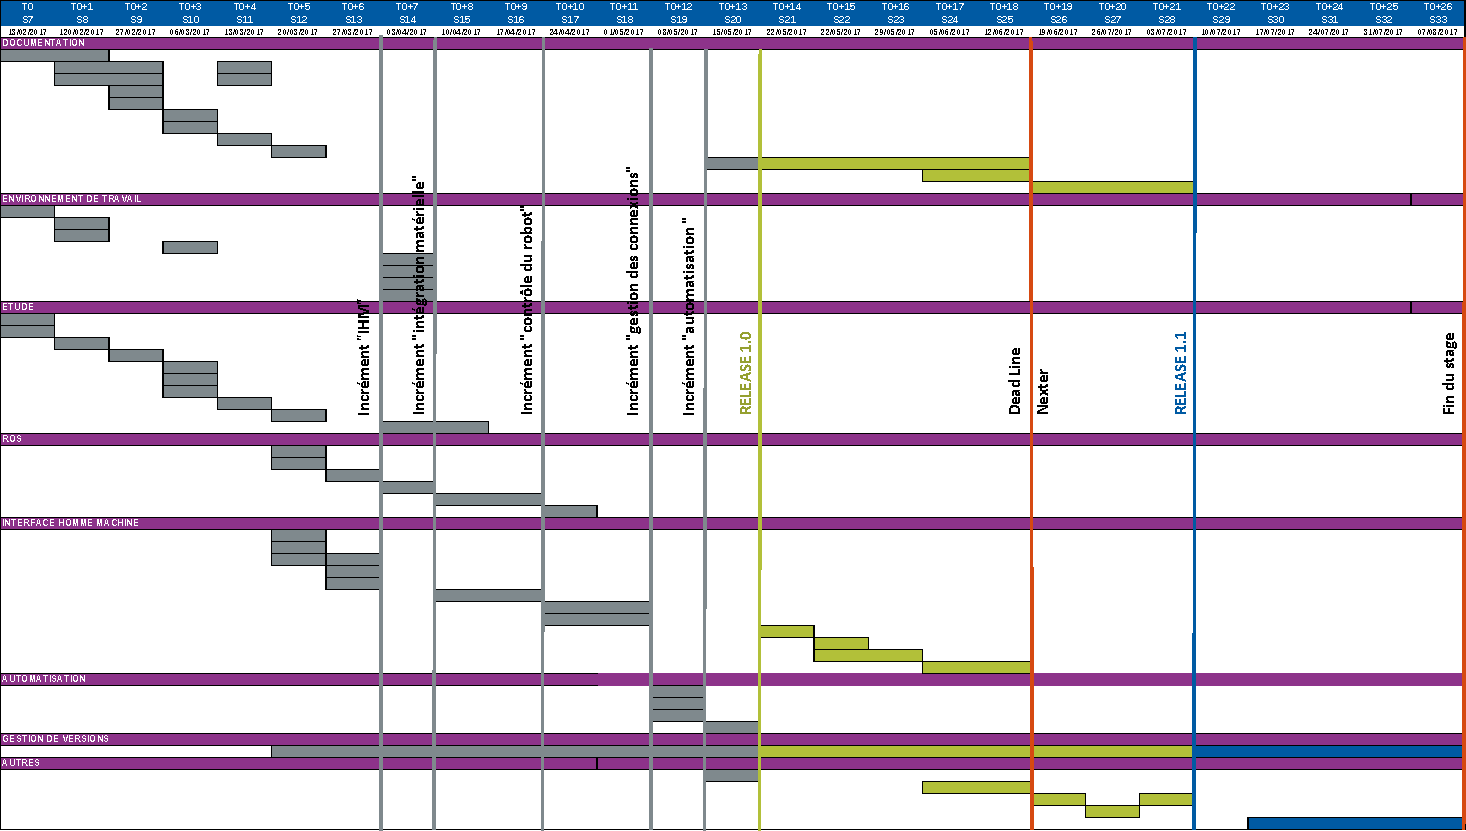
\includegraphics[width=1.\linewidth]{figures/planning-overview}  
    \captionof{figure}{Aperçu du planning complet, jalons et dead-lines clés, sans la dénomination des tâches}
  \label{fig:planning-overview}
\end{sidewaysfigure}

\begin{sidewaysfigure}
\centering
    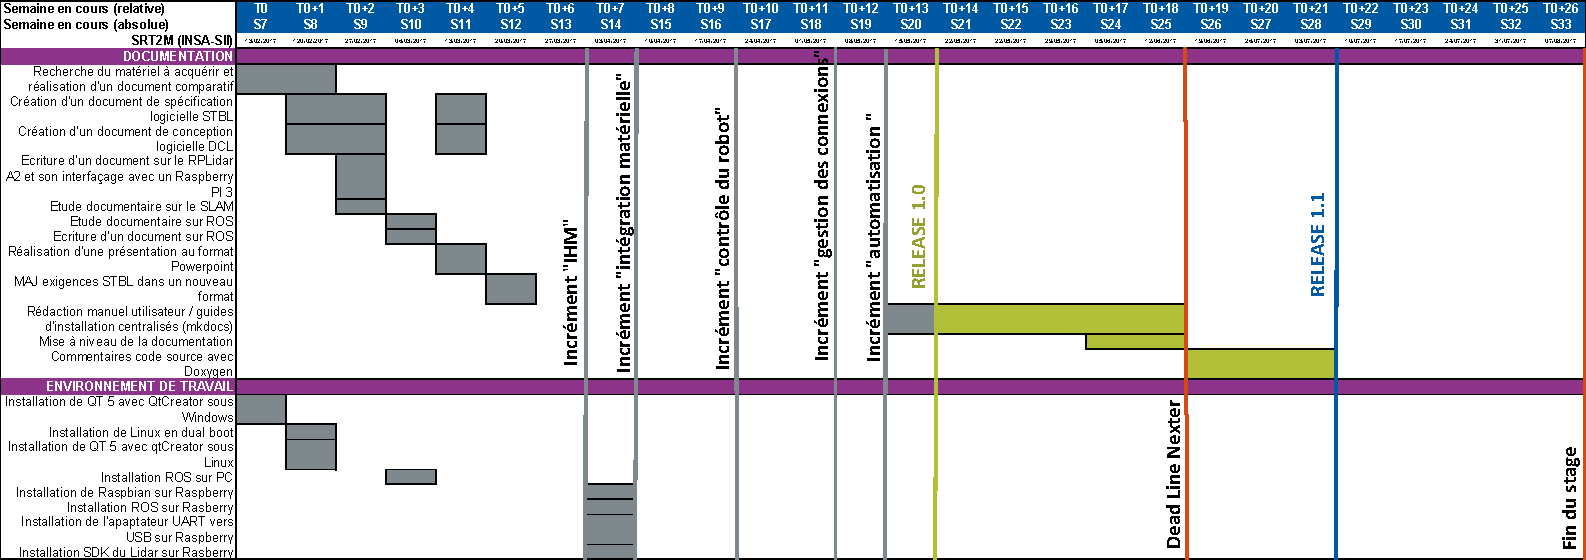
\includegraphics[width=1.\linewidth]{figures/Planning-1}  
    \captionof{figure}{Détail du planning, partie 1}
  \label{fig:planning-1}
\end{sidewaysfigure}

\begin{sidewaysfigure}
\centering
    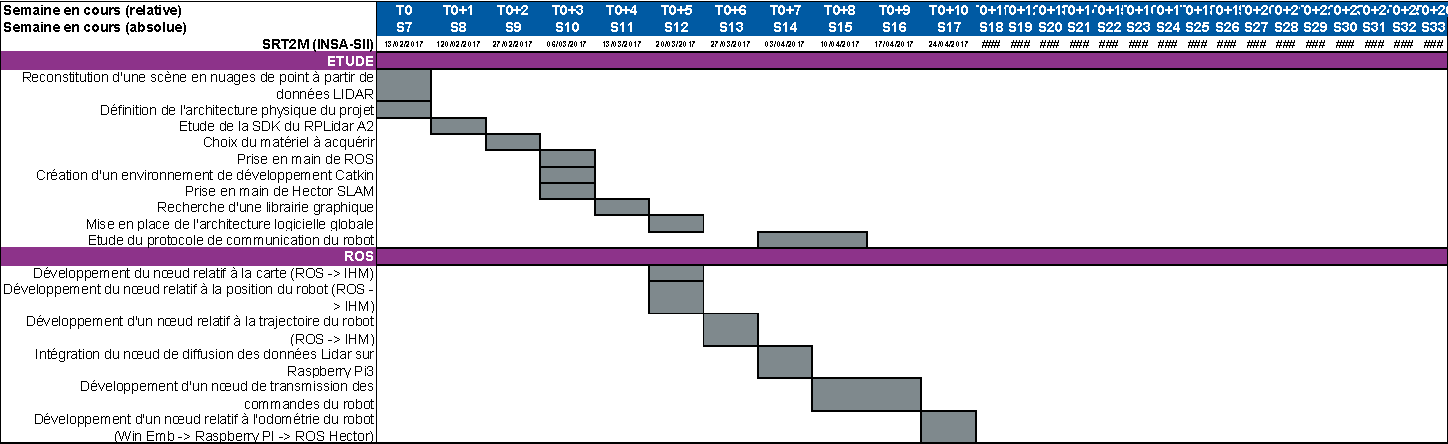
\includegraphics[width=1.\linewidth]{figures/Planning-2}  
    \captionof{figure}{Détail du planning, partie 2}
  \label{fig:planning-2}
\end{sidewaysfigure}

\begin{sidewaysfigure}
\centering
    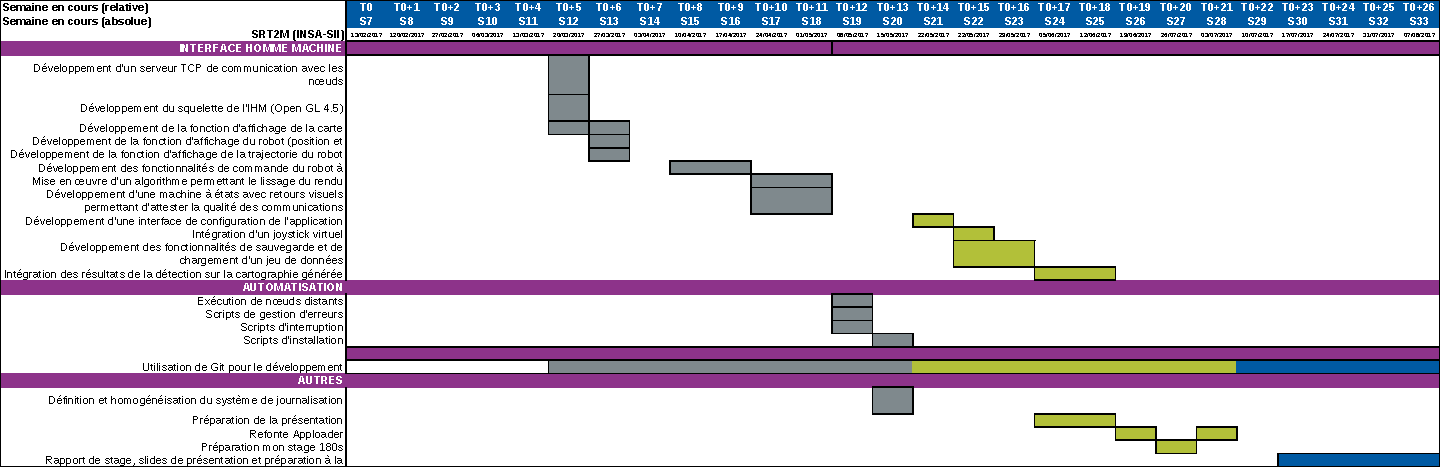
\includegraphics[width=1.\linewidth]{figures/Planning-3}  
    \captionof{figure}{Détail du planning, partie 3}
  \label{fig:planning-3}
\end{sidewaysfigure}